
%\documentclass[10pt,twoside,twocolumn]{article}
\documentclass[12pt,twoside]{article}
\usepackage[bf,small]{caption}
\usepackage[letterpaper,hmargin=1in,vmargin=1in]{geometry}
\usepackage{paralist} % comapctitem, compactdesc, compactenum
\usepackage{titlesec}
\usepackage{titletoc}
\usepackage{times}
\usepackage{hyperref}
\usepackage{algorithmic}
\usepackage{graphicx}
\graphicspath{{./graphics/}}
\usepackage{xspace}
\usepackage{verbatim}
\usepackage{url}
\usepackage{float}
\hyphenation{Sub-Bytes Shift-Rows Mix-Col-umns Add-Round-Key}

\setlength{\parskip}{12pt}
\setlength{\parindent}{0pt}

\newcommand \hdb {\textit{hashdb}\xspace}
\newcommand \sscope {\textit{SectorScope}\xspace}
\newcommand \aut {\textit{Autopsy}\xspace}
\newcommand \bulk {\textit{bulk\_extractor}\xspace}

\newcommand{\hb}{\emph{HBase}\xspace}
\newcommand{\fm}{\emph{Feature Miner}\xspace}
\newcommand{\ffm}{\emph{Forensic Feature Miner}\xspace}

\begin{document}

\begin{center}
\Large Design considerations for an HBase feature scanner\\
\end{center}

Proposed project name: \fm or \ffm

This paper provides a log of design considerations toward creating an HBase feature scanner.

\section{\fm Capabilities}
\begin{compactitem}
\item Rapidly ingest features from media images into an HBase data store.
\item Easily add media images into an HBase data store.
\item Store multiple feature classes: email addresses, facebook data, more.
\item Perform TF-IDF and other analytics on feature classes.
\item Perform TF-IDF and other analytics from a desktop client.
\end{compactitem}

\section{The Data Store}
The data store must fill these requirements:
\begin{compactitem}
\item Scalable to billions of records.
\item Distributed across a compute cluster.
\item Organized for efficient storage/retrieval.
\item Fault tolerant.
\end{compactitem}

A data record is defined as:\\
\texttt{Row Key, Col Family, Col Qualifier $=$ Value}\\

Data records consist of:
\begin{compactitem}
\item \textbf{Row Key} - The key used to retrieve this row of data. We use the feature class, for example \texttt{email}, followed by a comma followed by the feature text, for example \texttt{someone@somewhere.com}.
\item \textbf{Column Key} - Column information, consisting of \textbf{Column Family} and \textbf{Column Qualifier}.
  \begin{compactitem}
  \item \textbf{Column Family} - Not used, we use \texttt{f}. A family name can delineate column categories such as columls with different compression requiremtnts or access requirements.
  \item \textbf{Column Qualifier} - The column name.  We use it to store the (media iamge name, media image offset) tuple identifying a location where the feature is found, for example \texttt{myimage,1000}.
  \end{compactitem}
\item \textbf{Value} - The value for the data record.  The value provides feature context. For email, this is the actual bytes of the email address plus some bytes before and after it. Note that we store the value even though it can be retrieved by knowing the feature class and location of the feature.
\end{compactitem}

\section{Storage}
HBase describes data records as a sparse table. Internally, HBase is a collection of (key, value) pairs. We store (key, value) records as (feature, feature metadata) tuples where the key is the feature as a (feature class, feature text) tuple, and the value is a (feature location, feature context) tuple.

For one column family, which is what we have, HBase stores these (key, value) data records in one file.
When the file gets too large ($>$8GB), HBase splits it in two based lexicographically on the row key.  HBase does not split records for the same key across files, so we need to make sure our rows do not get larger than 8GB.  So for example if we have an email row with one million 200-byte columns, it will consume 200MB, which is much less than 8GB, so this is fine.

\section{Lookup}
\subsection{Filters}
We retrieve specific rows of the store based on specific filters we provide. Filters work by applying comparators (such as $=$ or $<$) to parts of the data record (such as Column Qualifier).  Pre-built filters work on bytes. If needed, we can write custom filters that convert bytes to data structures and compare data structures.

\subsection{Whole-class Analysis}
For analyzing all data in a class, such as all email addresses, we iterate over every record in the store, which can be slow. To mitigate this, we do the following:

\begin{compactitem}
\item We use filters that run on the data servers and return a list of rows to the requesting client (watch out for requesting too large of a list).
\item We may find a scatter/gather strategy for analyzing data on servers and then collating results on the client.
\end{compactitem}

\section{Client usability}
\begin{compactitem}
\item The end user will want to issue canned queries and will not want to make their own.
\item The end user will want to issue queries from a remote desktop.
\item Our solution should be generic so that \fm serves as a design model for other big-data tools.
\end{compactitem}

\section{February 7, 2017}
We want to support similarity and contiguity.  We pick email addresses for our discussion:

\begin{compactitem}
\item \textbf{Similarity} - Email addresses have similarity if they are identical but appear in different places. The key is the email address and the values are the columns containing (image, offset) tuples of places containing that email address.
\item \textbf{Contiguity} - Email addresses have contiguity if they are separated by similar data.  The key is the location (image, offset tuple) of an email address.  The values are email addresses nearby.
\end{compactitem}

\subsection{Defining Contiguity}
An approach discussed is to track the MD5 of the block containing an email address.  Adjacent email addresses on other drives would be in blocks adjacent to the block with the MD5.

The problem with this is that blocks across the media image are ordered by file and nothing else.  When blocks adjacent to a matching MD5 block do not match, this indicates that the blocks are from different files and thus are totally irrelated.  The file-based similarity section proposes a filesystem-based analysis rather than a raw-block analysis.

\subsection{Vocabulary}
\begin{compactitem}
\item \textit{Feature} changes to \textit{Artifact}.  \bulk features are forensic artifacts.
\item \textit{Feature type} changes to \textit{Class} to be in line with data classification, for example email class or facebook ID class.
\end{compactitem}

\section{Finding Similarity between Media Images}
This section presents several approaches for identifying cross-drive similarity:
\begin{compactitem}
\item Artifact similarity based on file membership.
\item Media image similarity based on data similarity, specifically, matching data blocks.
\item Artifact similarity based on byte proximity.
\item Cross-drive artifact similarity.
\end{compactitem}


\subsection{Artifact Similarity Based on File Membership}
This section proposes a file-based three-tiered many-to-many bimap lookup scheme for finding cross-drive artifact similarity as shown in Figure \ref{fig:threeTierBimap}.

\begin{figure}
	\center
	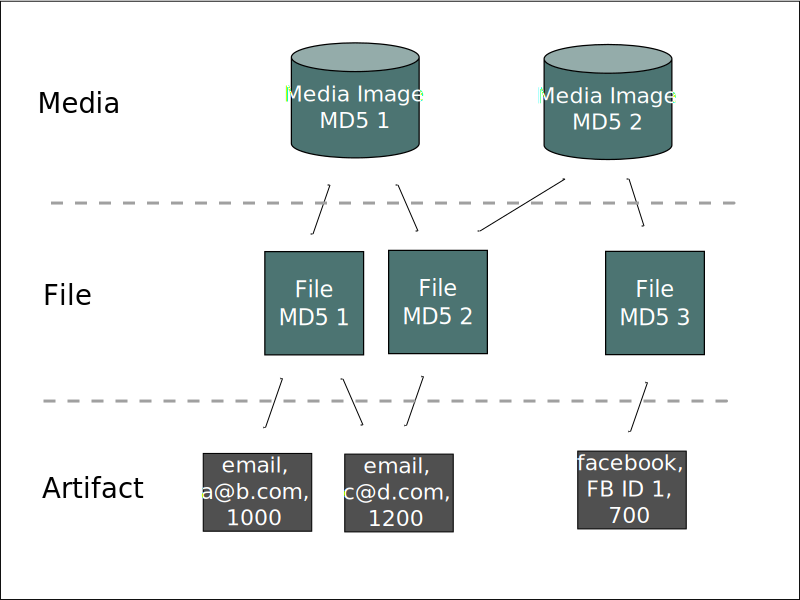
\includegraphics[scale=.45]{three_tier_bimap}
	\caption{Three-tier bimap for detecting artifact similarity}
	\label{fig:threeTierBimap}
\end{figure}

The three tiers are:
\begin{compactitem}
\item Media images, identified by their MD5.
\item Files, identified by their MD5.
\item Artifacts, identified by tuple (artifact class, artifact content, artifact offset), for example \texttt{email,a@b.com, 1000}.
\end{compactitem}

The bimaps are implemented as four (key, value) maps:
\begin{compactitem}
\item \verb+media_to_file+ maps media image MD5 values to filename MD5 values for all files in the media image.
\item \verb+file_to_media+ maps filename MD5 values to media image MD5 values for all media images containing the file.
\item \verb+file_to_artifact+ maps filename MD5 values to (class, artifact, offset) artifact tuples.
\item \verb+artifact_to_file+ maps (class, artifact, offset) tuples to filename MD5 values. Note that the artifact tuples are lexicographically ordered. This allows ordered lookup of filename MD5 values when the offset field is not needed.
\end{compactitem}

An example search is: What media images contain email address \verb+a@b.com+ and all email addresses adjacent to \verb+a@b.com+ in file MD5 1?

\begin{enumerate}
\item Get the list of email addresses in file MD5 1.
\item For each email address in the list: get the list of associated file MD5 values.
\item For each file MD5 value in the list: get the list of associated media iamge MD5 values.
\item Return the list of associated media image MD5 values.
\end{enumerate}

\subsection{Media Image Similarity}
We can detect media image similarity by comparing similar blocks between media images using media and block MD5 hashes as shown in Figure \ref{fig:blockSimilarity}.  We store a bimap between media image MD5 values and block MD5 values. We choose 512-byte blocks rather than 4K or larger blocks because file systems can align blocks along a 512-byte offset skew.

\begin{figure}
	\center
	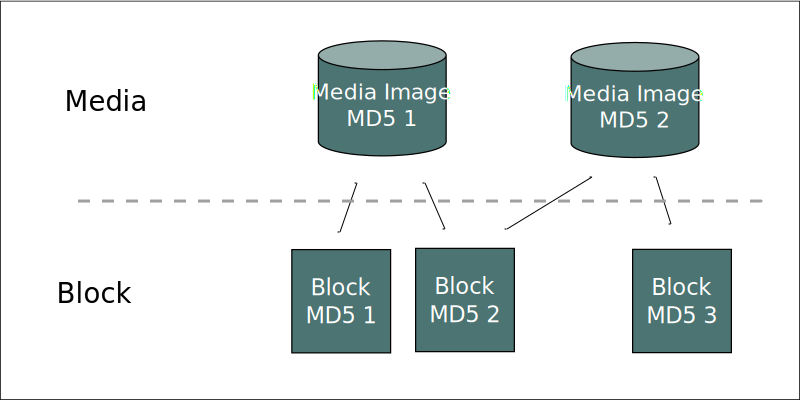
\includegraphics[scale=.45]{block_similarity}
	\caption{Bimap for detecting block similarity}
	\label{fig:blockSimilarity}
\end{figure}

The bimap consists of two (key, value) maps:
\begin{compactitem}
\item \verb+media_to_block+ maps media image MD5 values to block MD5 values:
  \begin{compactitem}
  \item Key: media image MD5.
  \item Data: tuple (block MD5, offset).
  \end{compactitem}
\item \verb+block_to_media+ maps block MD5 values to media image MD5 values:
  \begin{compactitem}
  \item Key: block MD5.
  \item Data: tuple (media image MD5, offset). To be compatible with scalability, blocks of all-zero bytes are skipped.
  \end{compactitem}
\end{compactitem}

We use \verb+media_to_block+ to get the list of blocks associated with a media image.
We use \verb+block_to_media+ to get the list of media images associated with a block.

The HBase implementation follows:
\begin{compactitem}
\item \verb+media_to_block+
  \begin{compactitem}
  \item Row Key: media image MD5 hexdigest + offset / 1 trillion. The offset / 1 trillion part splits the key to manageable sizes so that its record size is less than 8GB.
  \item Column Family: \verb+f+.
  \item Column Key: block MD5 hexdigest + offset.
  \item Cell: \verb+""+.
  \end{compactitem}
\item \verb+block_to_media+
  \begin{compactitem}
  %\item Row Key: block MD5 hexdigest + first two bytes of media image MD5 hexdigest. The extra bytes splits the key to manageable sizes so that the largest record sizes should be less than 8GB.
  \item Row Key: block MD5 hexdigest
  \item Column Family: \verb+f+.
  \item Column Key: media image MD5 + offset.
  \item Cell: \verb+""+.
  \end{compactitem}
\end{compactitem}

\subsection{Artifact Similarity Based on Byte Proximity}
In this approach, we identify artifact relations based on artifact closeness. For example we may say two artifacts are related if they are within 1,000 bytes of each other.

Note that this approach is different from a file-based approach where artifacts are related if they are in the same file. Here are some differences:

\begin{compactitem}
\item Processing contiguous sectors is more efficient than processing files.
\item Processing contiguous sectors catches artifacts in free-space.
\item Processing contiguous sectors can produce false positives when artifacts are in adjacent sectors but are not in the same file.
\end{compactitem}

This approach uses one map which maps (image, offset) tuples to artifacts as shown in Figure \ref{fig:offsetSimilarity}. The map is implemented using (key, value) pairs as follows:

\begin{figure}
	\center
	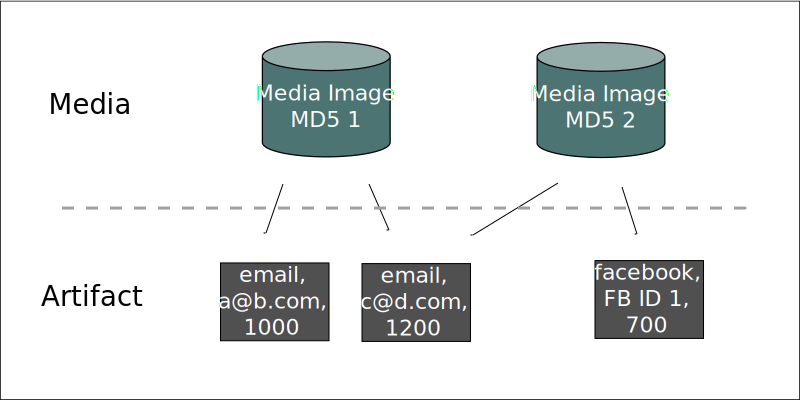
\includegraphics[scale=.45]{offset_similarity}
	\caption{Map for detecting artifact similarity}
	\label{fig:offsetSimilarity}
\end{figure}

\begin{compactitem}
\item \verb+image_to_artifact+ maps (image, offset / 1 trillion) tuples to (class, artifact, offset) tuples.
\end{compactitem}

Once the map is populated, feature similarity within a media is calculated by iterating through the values for adjacent artifacts.

\subsection{Cross-drive Artifact Similarity}
We find drives containing a provided email address. An email address can point to multiple offsets and multiple drives, as shown in Figure \ref{fig:artifactSimilarity}.

\begin{figure}
	\center
	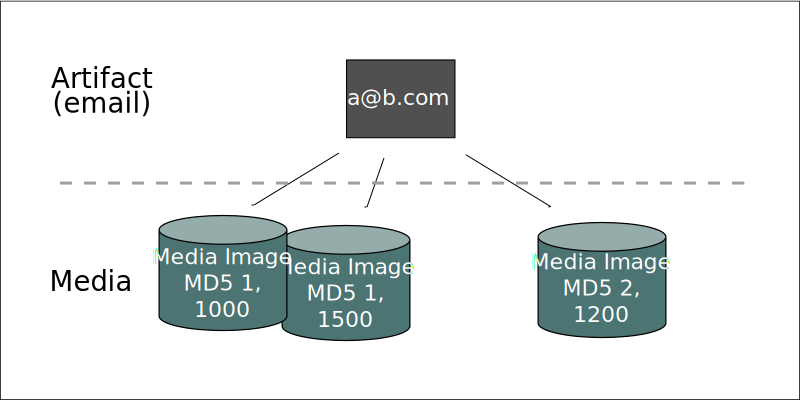
\includegraphics[scale=.45]{artifact_similarity}
	\caption{Map for detecting artifacts common across drives}
	\label{fig:artifactSimilarity}
\end{figure}

The data store consists of a map:
\begin{compactitem}
\item Key: email address.
\item data: tuple (media image MD5, offset).
\end{compactitem}

The HBase implementation consists of one table per artifact class. We describe the email artifact class:
\begin{compactitem}
\item \verb+email_to_image+
  \begin{compactitem}
  \item Row Key: email address, for example \verb+a@b.com+.
  \item Column Family: \verb+f+.
  \item Column Key: media image MD5 + offset.
  \item Cell: \verb+""+.
  \end{compactitem}
\end{compactitem}

Example usage: Find the top ten drives containing \verb+a@b.com+ and show the email frequency count for each.

\section{February 15, 2017}
\subsection{Problem with Slow Ingest}
During email ingest, compute nodes are using up free memory. The problem is the JVM Garbage Collector (GC) is not keeping up with recycling. To fix this, we must reduce how many objects are created during processing.

To start, we need to stop using JFlex because its grammar parsing generates too many temporary objects, \url{https://sourceforge.net/p/jflex/mailman/message/1109702/}.

Next, we need to not create a big array of objects that get pushed into the DB on a second pass; we need to push artifacts into the DB directly, without creating an interim array. The array costs by unnecessarily having objects to create/destroy and by having an extra layer of copying data.

Between these two improvements, GC should be in better control.

\subsection{JFlex Alternative}
I expect to replace the JFlex parser with a two-step scan process:
\begin{enumerate}
\item Iterate through data searching for potential artifacts.
\item For potential artifacts, run it through a regular epression parser. If valid, take it.
\end{enumerate}
For email addresses:
\begin{enumerate}
\item Iterate forward through data searching for a \verb+@+ token.
\item Expect unicode\_16 if the next byte is 0x00.
\item Step backward from \verb+@+ to find the start.
\item Step forward from \verb+@+ to find the end.
\item Run this range through a regular epression parser to check validity.
\item If valid, store the artifact.
\item Iterate one byte past this \verb+@+ token.  Repeat.
\end{enumerate}

\subsection{Replace HBase with Cassandra}
Article \url{https://www.linkedin.com/pulse/real-comparison-nosql-databases-hbase-cassandra-mongodb-sahu} shows that Cassandra is better for storing Forensic artifacts:
\begin{compactitem}
\item Performance is significantly faster.
\item Unlike HBase, Consistency is not guaranteed. But having a delay to achieve consistency is acceptable.
\item Both DBs are adequately supported as part of Apache.
\end{compactitem}

\section{February 23, 2017: \hdb Swap Space Bug}
\subsection{Problem}
\hdb v3.0.0 fails when adding large amounts of data.
This is detected on Linux-based systems.
The problem is that the amount of swap space available is
insufficient for LMDB.  This is a problem in particular for hashdb V3
which internally deletes data to add larger entry lists (V2 did not
delete anything).  From the LMDB article, it appears that swap space is
consumed when data is deleted.  LMDB never releases allocated virtual memory.\\

Being disk-backed, LMDB never frees allocations and grows really big, in
particular as a result of performing delete operations (I delete records
in order to put in replacement records that are longer as source offset
lists grow).

\subsection{Immediate Solution}
The immediate solution is to make the swap size really big.
The preferred solution is to redesign DB usage to not need swap.

\subsection{Localized Solution}
Being disk-backed, LMDB never frees allocations and grows really big, in
particular as a result of performing delete operations (I delete records
in order to put in replacement records that are longer as source offset
lists grow).

Additionally, the DB build process is slow.

In order to fix my swap-space exhaustion bug and to improve DB build
speed, I would like to discontinue storing all source offset values in
the Hash Data Store.  Currently, a configuration parameter allows us to
store up to 50 source offset values.  The change to the user will be as
if the option for storing zero source offset values was set.

Additionally, I would like to store source offset sub-counts in two
bytes, max 65535, instead of as variable-length protobuf numbers.  This
allows me to edit sub-count in place rather than jarring the DB with a
delete followed by a larger insert.  Recall that sub-count is the number
of times a hash has been seen in a particular source, while the total
count is the number of times a hash has been seen total, for all sources.

This change requires the user to get offsets to hashes within sources as
a separate operation if they actually need this value.

I believe this change will improve usability and that the loss of having
source offsets stored in the DB is acceptable.

\subsection{Distributed Solution}
This solution is proposed by Scott. From Scott:\\

I think you will have to shard the master database so that you can work within RAM on a cluster.  Each node would handle a shard of just hash\_data\_store, and the other tables are solely managed by the master.  From your master, on insert you create an "operation log" or "oplog" stream that is just a sequence of operations to be split out and played on each node.  Each operation would be a simple sequence like "insert sector X offset Y".  Since you are purely appending, this should not consume RAM.

Actually this could work on a single box.  Shard the oplog into separate files, then build each shard one-at-a-time.  Then you could do a merge operation if you want a single monolithic DB above RAM size.  Merges tend to iterate over the databases sequentially, so there should not be terrible random-access RAM pressure.

Also from Scott:\\
I think you can get a good design with the oplog.  Essentially you can do some work now, some work later so that you do not need to maintain a large memory state.  I could see the oplog as useful for a couple of reasons:

1. Sharding and Replicas.  You pipe only relevant data to the relevant nodes, or do "temporal sharding" where you create the shards sequentially on the same box one at a time.

2. Coalescing.  Sharding is like the first stage of a radix sort.  If you could cache operations before you flush them to the oplog, then you could get sorting and coalescing effects.  For example, you could maintain a list in memory of 100000 memory ops.  If you see the same address (for example, the all-0 block or another high-entropy but repetitive one) then you just increment its count and add it to a list in memory.  When you have memory pressure you flush this in-memory structure to the oplog, producing operations that say things like "increment count by 1234, add [source, [offsets]] to the DB" so part of the work creating the final DB state is accumulated before flushing.  It could also sort the data before flushing to the oplog, potentially making the data faster to merge into the database.


I have also been thinking of a multi-level "cache" on the read side too.  When creating hash-store via full table scan of hash-data-store, you could also create a smaller hash-store with the highest count items.  This small database could be copied to all the hasher nodes and used as a prefilter to reduce network traffic to the shards of the full hash-store.

My summary:\\
For oplog, ref: \url{https://docs.mongodb.com/manual/core/replica-set-oplog/}. An oplog could be used for error recovery.  Its operations are idempotent.

\subsection{Remove Source Offsets}
Either way, removing source offsets from the store would be good because we figured out how to track count information without them. If required, source offsets can be recalculated from source data offline. \sscope and two other known use-cases do not require it.

\subsection{Remove the \texttt{source\_data\_manager insert} Operation}
The \verb+source_data_manager+ supports \verb+insert+ and \verb+merge+.
The \verb+insert+ function increments source count.
The \verb+merge+ function replaces source count.
By using an \textit{oplog}, an entire source file is processed up front, so \verb+insert+ is discontinued and is removed.

\section{March 1, 2017: C++ \bulk scanners through JNI}
Create big-data scanners that capture the same artifacts as \bulk:
\begin{compactitem}
\item Create \verb+libbe_scan.so+, This library will contain C++ \bulk scanners ported to work with Apache Spark and Cassandra.
\item Calls to \verb+libbe_scan+ include \verb+scan_email(byte[])+. The actual parameter list may include additional metadata such as filename and file offset.
\item Calls to \verb+libbe_scan+ will scan bytes and write artifacts in tables in the Cassandra DB, for example email will go to the email table.
\item In the future, recursive decompression will be supported. This will require tracking additional metadata for managing recursive forensic paths.
\end{compactitem}
%\subsection{The \texttt{be\_scan} Library}
Design:
\begin{compactitem}
\item \verb+libbe_scan.so+ will compile on *nix systems using \textit{GNU Autotools}. The design will reflect that of \bulk and \hdb.
\item The Java JNI bindings will be built using SWIG. A proof-of-concept prototype is available in the \verb+jni_test+ directory. Note that \hdb uses SWIG for its Python bindings.
\end{compactitem}

\subsection{March 2, 2017: API Option}
We have a choice of layer for the API:
\begin{compactitem}
\item All at once: call one \verb+scan_all()+ function.  The C++ code will open the HDFS file, read the split, and perform all scans.
\item One per scanner: call \verb+scan_<artifact class>()+ for each artifact type, for example email. Java will read the split and pass the \verb+byte[]+ pointer to each scanner.
\end{compactitem}
We will have an API interface for each scanner. These interfaces will accept metadata requisite for handling recursion and forensic paths.
There will also be an initialization interface for Cassandra setup, \verb+open()+. These interfaces will be static, node-local, and threadsafe per Cassandra thread safety.

\end{document}

